\RequirePackage{fix-cm} % fix some latex issues see: http://texdoc.net/texmf-dist/doc/latex/base/fixltx2e.pdf
\documentclass[ twoside,openright,titlepage,numbers=noenddot,headinclude,%1headlines,% letterpaper a4paper
                footinclude=true,cleardoublepage=empty,abstractoff, % <--- obsolete, remove (todo)
                BCOR=5mm,paper=a4,fontsize=11pt,%11pt,a4paper,%
                ngerman,american,%
                ]{scrreprt}
\PassOptionsToPackage{usenames,dvipsnames}{xcolor}%needed because several packages include xcolor
\PassOptionsToPackage{utf8}{inputenc}
\usepackage{inputenc}
\PassOptionsToPackage{eulerchapternumbers,listings,%drafting,%
					 pdfspacing,%floatperchapter,%linedheaders,%
					 subfig,beramono,eulermath,parts}{classicthesis}                                        
\usepackage{url}
\usepackage{nameref}
\usepackage{datetime} %needed to add the date just below
\usepackage{pdflscape} %used to rotate pages with wide tables
\usepackage{rotating} %used to rotate wide figures
\usepackage{siunitx} %used for nice number formatting
\usepackage{pgf} % needed for arrays among other things

\def\authors{
  {Ivan Luchev, 201303660}}
\def\myTitle{Decentralized Storage System With Verification\xspace}
\def\mySubtitle{\xspace}
\def\myDegree{Project Report\xspace}
\def\myShortNames{Ivan Luchev\xspace}
\def\myGroup{}
\def\myProf{Niels Olof Bouvin\xspace}
\def\myOtherProf{\xspace}
\def\mySupervisor{\xspace}
\def\myFaculty{Faculty of Natural Sciences\xspace}
\def\myDepartment{Department of Computer Science\xspace}
\def\myUni{Aarhus University\xspace}
\def\myLocation{Aarhus\xspace}
\def\myTime{\monthname\ \the\year\xspace}
\def\myVersion{\xspace}


% ********************************************************************
% Setup, finetuning, and useful commands
% ********************************************************************
\newcounter{dummy} % necessary for correct hyperlinks (to index, bib, etc.)
\newlength{\abcd} % for ab..z string length calculation
\providecommand{\mLyX}{L\kern-.1667em\lower.25em\hbox{Y}\kern-.125emX\@}
\providecommand{\mBibTeX}{\textsc{Bib}\negthinspace\TeX\@}
% ****************************************************************************************************


% ****************************************************************************************************
% 3. Loading some handy packages
% ****************************************************************************************************
% ******************************************************************** 
% Packages with options that might require adjustments
% ******************************************************************** 
%\PassOptionsToPackage{ngerman,american}{babel}   % change this to your language(s)
% Spanish languages need extra options in order to work with this template
%\PassOptionsToPackage{spanish,es-lcroman}{babel}
\usepackage[american]{babel}                  
\usepackage{microtype}
\usepackage{csquotes}
\usepackage{ragged2e}
% \usepackage[usenames,dvipsnames]{xcolor}
\usepackage{xcolor}
\usepackage{pgf-umlsd}
\usepackage{pgfplots}
\usepackage{pgfplotstable}
% recommended:
\usepackage{booktabs}
\usepackage{array}
\usepackage{colortbl}
% \usepackage{color}
\definecolor{aublue}{HTML}{193b77} % the dark blue colour used by AU



\usepackage{helvet}
\usepackage{etoolbox}
\usepackage{graphicx}
\usepackage{caption}
\usepackage{booktabs}
\usepackage[usenames, dvipsnames]{xcolor} 
\usepackage{setspace}
\usepackage{amsthm}
\usepackage{xparse}
\usepackage{hyperref}
\usepackage{amssymb} % for mathbb
\usepackage{soul} % for highlighting
    \definecolor{highlight}{gray}{0.85}
    \sethlcolor{highlight}
\usepackage[many]{tcolorbox} % for boxes definitions
\usepackage[all]{xy} % for xy-matrix
\usepackage{algpseudocodex} % for algorithm set-up
\renewcommand{\c}[1]{\mathcal{#1}}
\renewcommand{\b}[1]{\boldsymbol{#1}}
\newcommand{\M}{\mathrm{M}}
\newcommand{\F}{\mathrm{F}}
\newcommand{\MT}{\mathsf{MT}}
\newcommand{\DPoR}{
    (\texttt{Init},\, \mathtt{Read},\, \mathtt{Write},\, \mathtt{Audit},\, \mathtt{Extract})
}
\newcommand{\Prob}{\mathbb{P}}
\newenvironment{changemargin}[2]{%
\begin{list}{}{%
\setlength{\topsep}{0pt}%
\setlength{\leftmargin}{#1}%
\setlength{\rightmargin}{#2}%
\setlength{\listparindent}{\parindent}%
\setlength{\itemindent}{\parindent}%
\setlength{\parsep}{\parskip}%
}%
\item[]}{\end{list}}
\newenvironment{definition}[1][]
    {\begin{tcolorbox}[%
        enhanced, 
        breakable,
        skin first=enhanced,
        skin middle=enhanced,
        skin last=enhanced,
        colback=white,
        ]
    \textbf{Definition.} (#1)
    \tcblower
    }{
    \end{tcolorbox}
    }

\definecolor{light_gray}{gray}{0.95}
\newenvironment{MATH}[2][]
    {\begin{tcolorbox}[%
        enhanced, 
        breakable,
        skin first=enhanced,
        skin middle=enhanced,
        skin last=enhanced,
        colback=light_gray,
        ]
    \textbf{#1.} (#2)
    \tcblower
    \begin{changemargin}{1cm}{1cm}
    }{
    \end{changemargin}
    \end{tcolorbox}
    }
\usepackage{tikz}
\usetikzlibrary{decorations.shapes}
\tikzset{
  decoration = {shape backgrounds, shape=circle,
                shape size=0.75pt, shape sep=4pt},
paint/.style = {decorate, fill=black}
}
\newtcolorbox{dottedBox}{%
enhanced,
breakable,
sharp corners,
boxrule=2pt,boxsep=0pt,top=4pt,left=4pt,right=4pt,bottom=4pt,middle=0pt,
colback=white,
colframe=white,
pad at break=0pt,bottomrule at break=0pt,toprule at break=0pt,
borderline={0pt}{0pt}{paint},
}%
\renewcommand{\footnotesize}{\fontsize{9}{11}\selectfont}
\usepackage{caption}
\usepackage{float}
\graphicspath{ {./Images/} }
\makeatletter
\patchcmd{\@maketitle}{\LARGE \@title}{\fontsize{16}{19.2}\selectfont\@title}{}{}
\makeatother
\date{}    

\usepackage{amsmath} % for math environments and operations
\usepackage{bm}      % for bold symbols in math mode

%\usepackage[square,numbers,sort&compress]{natbib}
%\bibliographystyle{abbrvnat}

\PassOptionsToPackage{%
   %backend=biber, %instead of bibtex
	backend=bibtex8,bibencoding=ascii,%
	language=auto,%
	style=numeric-comp,%
   %style=authoryear-comp, % Author 1999, 2010
   %bibstyle=authoryear,dashed=false, % dashed: substitute rep. author with ---
   sorting=nyt, % name, year, title
   maxbibnames=10, % default: 3, et al.
   %backref=true,%
   natbib=true % natbib compatibility mode (\citep and \citet still work)
}{biblatex}
\usepackage{biblatex}


\PassOptionsToPackage{fleqn}{amsmath}       % math environments and more by the AMS 
\usepackage{amsmath}
%
% ******************************************************************** 
% General useful packages
% ******************************************************************** 
\PassOptionsToPackage{T1}{fontenc} % T2A for cyrillics
\usepackage{fontenc}     
\usepackage{textcomp} % fix warning with missing font shapes
\usepackage{scrhack} % fix warnings when using KOMA with listings package          
\usepackage{xspace} % to get the spacing after macros right  
\newcommand{\eg}{e.g.,\xspace}
\newcommand{\Eg}{E.g.,\xspace}
\newcommand{\etal}{et~al.\xspace}
\newcommand{\etc}{etc.\@\xspace}
\newcommand{\ie}{i.e.,\xspace}
\newcommand{\viz}{viz.\@\xspace}

\usepackage{mparhack} % get marginpar right
\usepackage{fixltx2e} % fixes some LaTeX stuff --> since 2015 in the LaTeX kernel (see below)
%\usepackage[latest]{latexrelease} % will be used once available in more distributions (ISSUE #107)
\PassOptionsToPackage{printonlyused,smaller}{acronym} 
    \usepackage{acronym} % nice macros for handling all acronyms in the thesis
    %\renewcommand{\bflabel}[1]{{#1}\hfill} % fix the list of acronyms --> no longer working
    %\renewcommand*{\acsfont}[1]{\textsc{#1}} 
    \renewcommand*{\aclabelfont}[1]{\acsfont{#1}}
% ****************************************************************************************************


% ****************************************************************************************************
% 4. Setup floats: tables, (sub)figures, and captions
% ****************************************************************************************************
\usepackage{tabularx} % better tables
    \setlength{\extrarowheight}{3pt} % increase table row height
\newcommand{\tableheadline}[1]{\multicolumn{1}{c}{\spacedlowsmallcaps{#1}}}
\newcommand{\myfloatalign}{\centering} % to be used with each float for alignment
\usepackage{caption}
% Thanks to cgnieder and Claus Lahiri
% http://tex.stackexchange.com/questions/69349/spacedlowsmallcaps-in-caption-label
% [REMOVED DUE TO OTHER PROBLEMS, SEE ISSUE #82]    
%\DeclareCaptionLabelFormat{smallcaps}{\bothIfFirst{#1}{~}\MakeTextLowercase{\textsc{#2}}}
%\captionsetup{font=small,labelformat=smallcaps} % format=hang,
\captionsetup{font=small} % format=hang,
\usepackage{subfig}  
% ****************************************************************************************************


% ****************************************************************************************************
% 5. Setup code listings
% ****************************************************************************************************
\usepackage{listings} 
%\lstset{emph={trueIndex,root},emphstyle=\color{BlueViolet}}%\underbar} % for special keywords
\lstset{language=[LaTeX]Tex,%C++,
    morekeywords={PassOptionsToPackage,selectlanguage},
    keywordstyle=\color{RoyalBlue},%\bfseries,
    basicstyle=\small\ttfamily,
    identifierstyle=\color{NavyBlue},
    commentstyle=\color{Green}\ttfamily,
    stringstyle=\rmfamily,
    numbers=left,
    numberstyle=\tiny\color{Gray},
    stepnumber=1,
    numbersep=8pt,
    showstringspaces=false,
    breaklines=true,
    %frameround=ftff,
    %frame=single,
    belowcaptionskip=.75\baselineskip
    %frame=L
} 



% ****************************************************************************************************             


% ****************************************************************************************************
% 6. PDFLaTeX, hyperreferences and citation backreferences
% ****************************************************************************************************
% ********************************************************************
% Using PDFLaTeX
% ********************************************************************
\usepackage{hyperref}
\PassOptionsToPackage{pdftex}{graphicx}
    \usepackage{graphicx} 

\usepackage{tcolorbox}

% ********************************************************************
% Hyperreferences
% ********************************************************************
\hypersetup{%
    colorlinks=true, linktocpage=true, pdfstartpage=3, pdfstartview=FitV,%
    breaklinks=true, pdfpagemode=UseNone, pageanchor=true, pdfpagemode=UseOutlines,%
    plainpages=false, bookmarksnumbered, bookmarksopen=true, bookmarksopenlevel=1,%
    hypertexnames=true, pdfhighlight=/O,%nesting=true,%frenchlinks,%
    urlcolor=webbrown, linkcolor=RoyalBlue, citecolor=webgreen, %pagecolor=RoyalBlue,%
    pdftitle={\myTitle},%
    pdfauthor={\textcopyright\ \myShortNames, \myUni, \myFaculty},%
}   

% ********************************************************************
% Setup autoreferences
% ********************************************************************
% There are some issues regarding autorefnames
% http://www.ureader.de/msg/136221647.aspx
% http://www.tex.ac.uk/cgi-bin/texfaq2html?label=latexwords
% you have to redefine the makros for the 
% language you use, e.g., american, ngerman
% (as chosen when loading babel/AtBeginDocument)
% ********************************************************************
\makeatletter
\@ifpackageloaded{babel}%
    {%
       \addto\extrasamerican{%
			\renewcommand*{\figureautorefname}{Figure}%
			\renewcommand*{\tableautorefname}{Table}%
			\renewcommand*{\partautorefname}{Part}%
			\renewcommand*{\chapterautorefname}{Chapter}%
			\renewcommand*{\sectionautorefname}{Section}%
			\renewcommand*{\subsectionautorefname}{Section}%
			\renewcommand*{\subsubsectionautorefname}{Section}%     
                }%
       \addto\extrasngerman{% 
			\renewcommand*{\paragraphautorefname}{Absatz}%
			\renewcommand*{\subparagraphautorefname}{Unterabsatz}%
			\renewcommand*{\footnoteautorefname}{Fu\"snote}%
			\renewcommand*{\FancyVerbLineautorefname}{Zeile}%
			\renewcommand*{\theoremautorefname}{Theorem}%
			\renewcommand*{\appendixautorefname}{Anhang}%
			\renewcommand*{\equationautorefname}{Gleichung}%        
			\renewcommand*{\itemautorefname}{Punkt}%
                }%  
            % Fix to getting autorefs for subfigures right (thanks to Belinda Vogt for changing the definition)
            \providecommand{\subfigureautorefname}{\figureautorefname}%             
    }{\relax}
\makeatother


% ****************************************************************************************************
% 7. Last calls before the bar closes
% ****************************************************************************************************
% ********************************************************************
% Development Stuff
% ********************************************************************
\listfiles
%\PassOptionsToPackage{l2tabu,orthodox,abort}{nag}
%   \usepackage{nag}
%\PassOptionsToPackage{warning, all}{onlyamsmath}
%   \usepackage{onlyamsmath}

% ********************************************************************
% Last, but not least...
% ********************************************************************
\usepackage{classicthesis} 

\def\myDegree{Decentralized storage system with verification}
\def\myTitle{Decentralized storage system with verification}
\def\mySubtitle{(KISS)}
\addbibresource{Bibliography}
\hyphenation{Micro-soft Web-RTC Chun-ky-Spread Ka-dem-lia Pas-try mac-OS block-chain time-stamp Et-he-re-um}

\begin{document}
\raggedbottom
\selectlanguage{american} % american
\pagenumbering{arabic}
\pagestyle{plain}
\include{FrontBackmatter/DirtyTitlepage}
\begingroup

\chapter*{Abstract}
KISS is a decentralized storage system with verification mechanisms.
The main goals of this system are to ensure durable replicated storage and to prevent or at least limit malicious peers' influence on the network.
In particular, attacks that aim to disrupt the integrity and storage guarantees of a decentralized storage system.
The system implements a key-value storage (aka. a distributed hash table) built on top of Kademlia in order
to provide logarithmic time for querying.
The nodes in the network are split into two kinds - one strictly storing files, and another taking care of indexing and validation.
The verifier nodes keep track of what files should be stored in the system and periodically verify that these files actually exist.
In other words the verifier nodes are the super-users of the system that keep track of which nodes behave correctly
and need to be rewarded or are malicious and need to be punished.
This reward-and-punishment mechanism is what keeps the system in check.
\vfill
\endgroup			

\chapter{Introduction}

TODO ... describe goals and expected results 

\chapter{Related Work}

Many decentralized storage systems have been proposed and implemented.
Modern distributed storage systems achieve up to logarithmic time for insert, lookup, and delete operations.
To name a few such systems - Chord \cite{chord}, Pastry \cite{pastry}, and Kademlia \cite{kademlia}.
The main difference between these systems is the way they organize the nodes in the network.
Chord and Pastry use a ring structure, while Kademlia uses a binary tree.
The ring structure is more efficient in terms of routing, but it is more difficult to maintain the ring structure
when nodes join and leave the network.
Kademlia is more resilient to churn, but it is less efficient in terms of routing.
Most of these systems serve as a foundation for applications that implement some kind of decentralized storage,
but we won't go into detail about them, because they are not the focus of this project.

There are also multiple proposals on how to make decentralized storage systems more resilient to malicious peers.
To name a few - ARA \cite{ara}, Tarzan \cite{tarzan}, and S/Kademlia \cite{skademlia}.
The main idea behind these proposals is to have some kind of auditing mechanism that checks if the peers are behaving correctly.
ARA proposes a system where peers share information about what data they are storing and check each other.
Tarzan focuses on anonymity of peers in the network by generating fake traffic and hiding the real traffic.
S/Kademlia focuses on node authentication with expensive node ID generation and verifiable messages using
public and private key cryptography.
S/Kademlia also routes requests through multiple different nodes at the same time
in order to reduce the chance of a request falling into a malicious subnet.

Comparison between performance between decentralized storage systems has been done before
\cite{kadvschordvspastry, 2019AIPC.2129b0131A}.
The results are that Pastry is the best performer for networks with under 1000 peers, but the paper also suggests
that Kademlia would probably outperform Pastry for larger networks.
The results in the 2 papers differ somewhat from the results in \cite{compstudy}, which suggests that theoretically
Chord should outperform Kademlia, but the paper does not do in-depth evaluation of networks with high churn rate
like \cite{kadvschordvspastry}.

\chapter{Architecture \& Implementation}
\label{cha:arch-impl}

\section{Architecture}
\label{sec:architecture}

The system is split into 2 components - Keeper and Verifier.
Keepers implement the Kademlia protocol and store the actual data,
while Verifiers keep track of what data should be stored and periodically verify that the data is still there.
In the current version there is one Verifier for simplicity reasons,
but in the future the Verifiers will be part of a p2p network as well.

The Keepers communicate between each other using the Kademlia protocol.
Kademlia is the backbone of the Keepers as it implements the peer discovery and routing.
All Kademlia communication is event-based and asynchronous.
In order to keep track of the Kademlia messages the Keepers use a local Hash Table.

The Verifiers communicate with the Keepers using GRPC.
This protocol was chosen because it is language agnostic and fast.
The Verifiers also use GRPC to communicate with the database - ImmuDB.

ImmuDB is an immutable database that uses Merkle trees to ensure data integrity.
The Verifiers use ImmuDB to store metadata about the files stored in the system.
The metadata includes the file name, and the hash of the file's content and the expiration date of the file.
The expiration date is used to determine when a file should be deleted from the system.
Deletion is implemented as a soft deletion - the Verifiers simply stop checking for the file's existence.

There was no library that implemented an API for ImmuDB in Rust and ImmuDB did not document how to create one,
so we had to reverse engineer the python library and implement a Rust library.
The Rust library is very limited as it implements only the necessary endpoints for this project.
The library is fairly simple as it performs a login request, which returns a token and then every
subsequent request uses this token to authenticate itself.

Below we can see a diagram of the process of saving a file in the system,
followed by a diagram of the process of retrieving a file from the system.

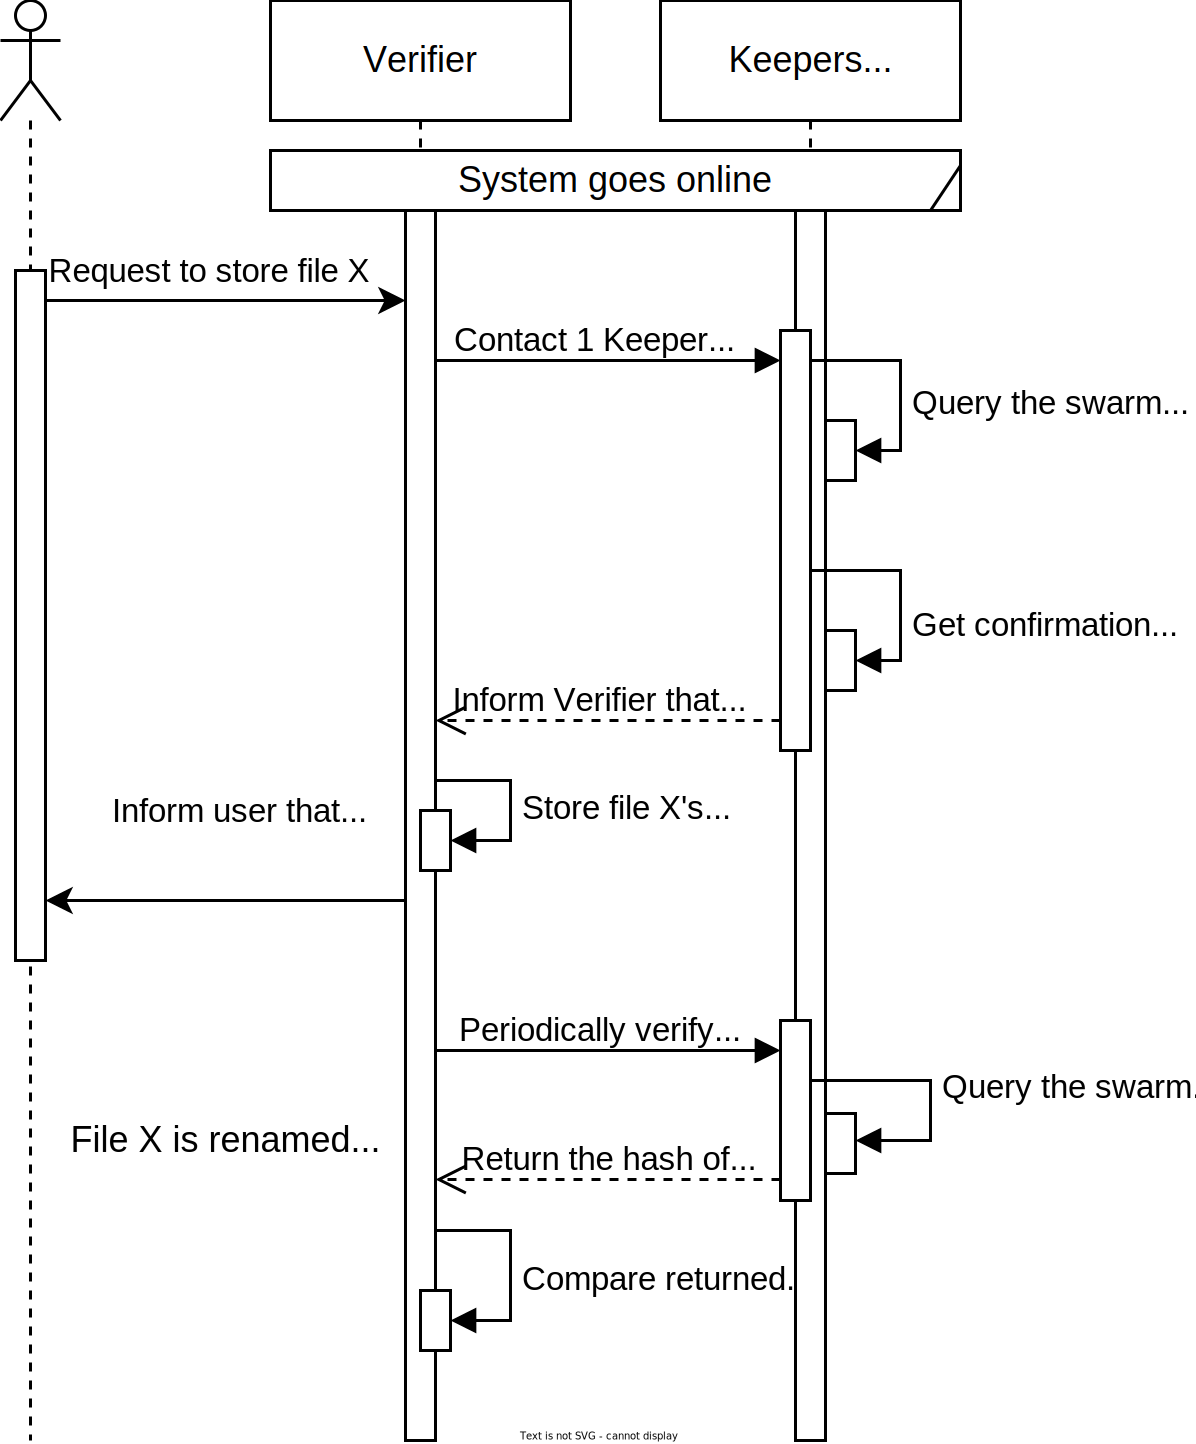
\includegraphics[width=350pt]{kiss-store}

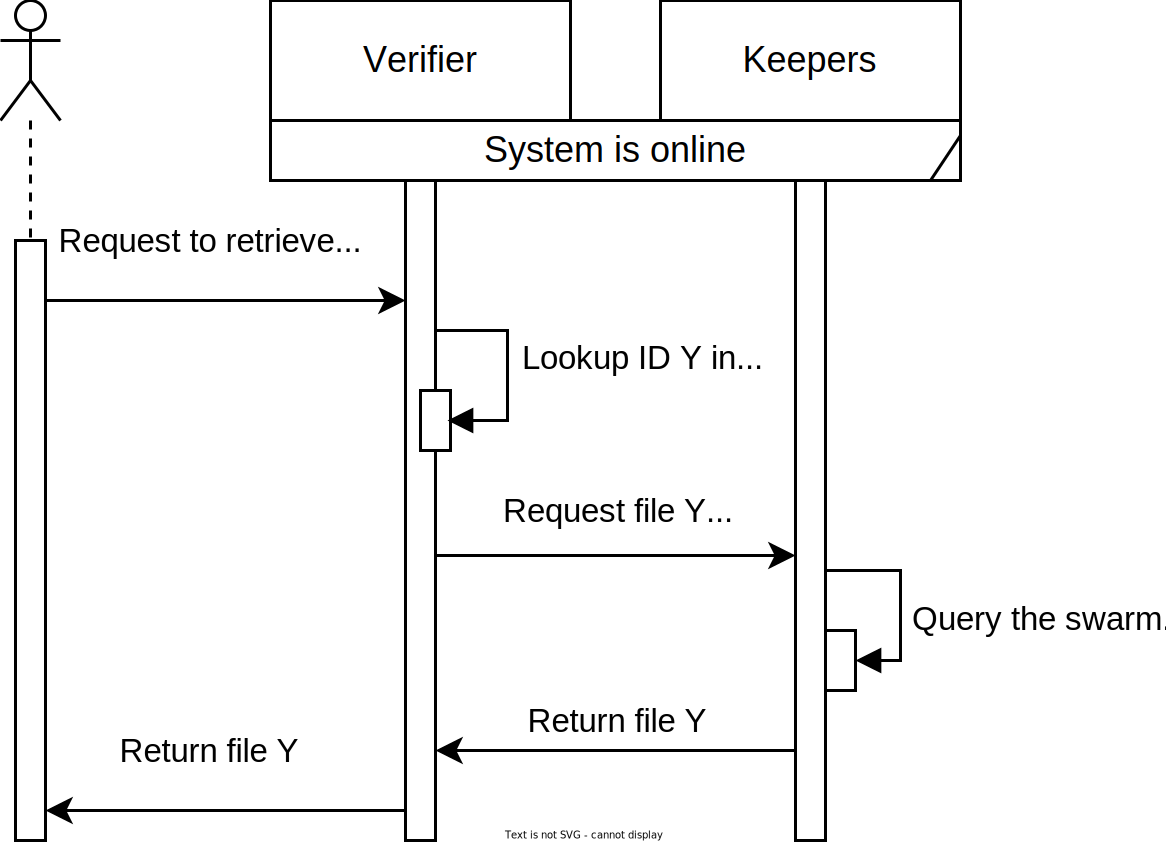
\includegraphics[width=350pt]{kiss-retrieve}


\section{Implementation}
\label{sec:implementation}

The system is implemented in Rust.
The main reason for this is that Rust is a systems programming language,
which means that it is fast and has a low memory footprint.
It also provides a lot of safety guarantees,
which is important for a system that needs to be resilient to malicious peers.

The common modules of the project containing constants and errors are separated in a separate library crate.
The custom errors are implemented using the error\_chain crate.
It provides a useful macro that allows to define custom errors with a description and a display message.
\begin{minted}{rust}
error_chain! {
    errors {
        ConfigErr(e: ConfigError) {
            description("loading config failed"),
            display("loading config failed: {}", e),
        }
    }
}
\end{minted}

This allows the custom errors to encapsulate any other errors from other crates.

Both the Keeper and the Verifier follow the same code architecture - asynchronous main with dependency injection
relying on yaml settings.

The main function looks similarly to:
\begin{minted}{rust}
async fn main() {
    match run().await {
        Ok(()) => info!("shutting down"),
        Err(err) => die(err), // prints the error and exits
    }
}
async fn run() -> Res<()> {
    env_logger::init(); // initialize the logger
    // initialize the dependency injector
    let injector = dependency_injector()?; 
    let grpc_handler: Svc<dyn IGrpcHandler> = injector.get();
    let kad: Svc<dyn ISwarm> = injector.get();
    // start the services asynchronously
    try_join!(grpc_handler.start(), kad.start())?;
}
\end{minted}

The logger has to be initialized before any other code is executed,
because the other code might use the logger.
The dependency injector is initialized next.
It lazily initializes the modules when one is requested for the first time, and caches the result.
For example, GrpcHandler depends on the Settings module,
so Settings will be initialized and then passed to GrpcHandler.
Finally, we start all modules and wait for them to error out.
The start methods are pretty much infinite loops that act as event listeners.

\begin{minted}{rust}
pub fn dependency_injector() -> Res<Injector> {
    let mut injector = Injector::builder();
    injector.add_module(p2p::module());
    injector.provide(
        SettingsProvider
            .singleton()
            .with_interface::<dyn ISettings>(),
            // Settings is an interface
    );
    injector.provide(
        KeeperGatewayProvider
            .singleton()
            .with_interface::<Mutex<KeeperGateway>>(),
            // No interface and no good concurrency :(
    );
    ...
}
\end{minted}

The dependency injector adds all dependencies as singletons.
This means that only one instance of each dependency will be created.
This is good because we ensure no different instances will try to access the same resource and cause a race condition.
But it also causes a huge pain to initialize some dependencies.
For example, the KeeperGateway module in the Verifier,
which is responsible for communicating with the Keepers over GRPC,
contains a Mutex<KeeperGrpcClient<\_> >.
This is needed because the GRPC client does not implement the necessary traits to be thread-safe and mutable.
Rust is very pedantic about having mutable variables being accessed from different threads,
so it disallows the GRPC client to be modified without a mutex.
So we have to wrap the GRPC client in a mutex, so we can provide the KeeperGateway as a singleton dependency.
But, if we want to take control of a mutex and modify the data inside, we need a mutable reference to it.
This means that the whole KeeperGateway needs to be mutable, i.e., provided in a mutex.
However, providing a module surrounded in a mutex breaks the idea of providing an interface,
because the mutex does not implement the KeeperGateway's interface.
We also cannot provide mutex surrounding an interface,
because the interface does not have a size known at compile time.

tl;dr; Rust is very pedantic about mutability and thread-safety,
which is good, but it makes it very difficult to use dependency injection in a multithreaded (async) environment.
We have to encapsulate modules, that are not implemented as thread-safe, into mutexes,
which makes them not implement the necessary interfaces, and that breaks the dependency injection idea.

Switching to something simpler - the Settings module reads off the settings from a YAML config file.
The Settings utilize the serde crate to deserialize the YAML file into a struct.
The config file specifies any variables that change between instances - for example the port number and any secrets.
Nothing fancy happens here.

The storage is pretty simple as well.
It uses the object\_store crate, which provides the necessary APIs to work with HDD storage or S3 storage.

The GRPC module is implemented using the tonic crate.
It is very well documented and explains in details how to implement a GRPC server and client.
It boils down to writing a protobuf definition and then tonic generates all the boiler-plate code,
leaving the developer to implement only the interface methods for the server and the client.

Another pretty hard to implement module is the Kademlia module.
The module itself is not hard to implement, but any interaction with the module is painful to say the least.
Kademlia is implemented with 1 field - Mutex<Swarm<CombinedBehaviour> >.
It has to be a mutex again, because this is the only way to provide it as a singleton,
and we need to have mutable access to the Swarm, so we can read events from it.
Where's the problem? Kademlia is initialized as an infinite loop that listens for events from the Swarm.
This means that we have to take a mutable reference to the Swarm and then pass it to the infinite loop.
Yes. The mutex is now locked, and we cannot access it from anywhere else.
The solution was to make a separate module, that - SwarmController,
which initializes a tunnel between itself and the Kademlia module,
that it uses to send messages to the Kademlia module.
i.e., These messages are the getters and setters of the Kademlia module.
And they are asynchronous, because we do not know when the Swarm will be unlocked or will not be processing
Kademlia events and will be ready to be used.
Here is how this looks in code:

\begin{minted}{rust}
async fn start(&self) -> Res<()> {
    let mut swarm = self.inner.lock().await;
    let mut receiver = self.swarm_controller.lock().await;
    loop {
        select! {
            instruction = receiver.recv() => {
                // handle controller (getter/setter) event
            },
            event = swarm.select_next_some() => {
                // handle kademlia event and
            }
        }
    }
}
\end{minted}

The select! macro allows us to wait for 2 blocking events and whenever 1 happens to execute the corresponding code.
Since this happens inside the Kademlia module, we can safely take ownership of the swarm (make it mutable).
This allows us to use the swarm and handle any Kademlia events at the same time.

The most excruciating part of the communication is how exactly
the SwarmController communicates with the Kademlia module.
I will try to put it into words, but it is very difficult to wrap one's head around it.
Here goes.

The SwarmController shares a two-way channel with the Kademlia module.
When someone calls the SwarmController getter a message is sent to the Kademlia module indicating
that a getter was called.
Kademlia does its p2p magic and whenever it receives a response from the Swarm it has to send back a message.
In order to achieve that in a non-blocking way the Kademlia module keeps a hash table with the IDs 
of the requests made to the swarm together with the way to send back a response.

Here's what the code in the SwarmController looks like for a getter:

\begin{minted}{rust}
async fn get(&self, key: String) -> Res<Bytes> {
    // Create a channel<channel>
    let (sender, receiver) = oneshot::channel::
        <OneReceiver<Res<Bytes>>>();
    self.swarm_api .send(SwarmInstruction::Get { key, resp: sender });
    // Get the channel where the response will be sent
    let receiving_channel = receiver.await.unwrap();
    // Get the actual response
    let result = receiving_channel.await.unwrap();
    result
}
\end{minted}

We send a channel containing a channel to the Kademlia module.
Next, the Kademlia module accepts the request and sends back a
channel where it will send the response when it receives it from the Swarm.
Kademlia also saves the channel where the response will be sent to the SwarmController
together with the ID of the request sent to the swarm in its hash table.
This happens in this piece of code:

\begin{minted}{rust}
async fn handle_controller_get<'t>(...) {
    let key = Key::new(&key);
    let (sender, receiver) = oneshot::channel::<Res<Bytes>>();
    // Send the channel receiver where the response will be
    // sent to the SwarmController
    resp.send(receiver).unwrap();

    let query_id = swarm.behaviour_mut().kademlia.get_record(key);
    // Add ID:sender-channel to the hash table
    self.queries.insert(query_id, QueryResponse::Get { sender });
}
\end{minted}

Finally, when the Kademlia module receives a response from the Swarm it sends it back to the SwarmController
over the channel, which was saved in the hash table in the previous code snippet.
Here's what the code looks like:

\begin{minted}{rust}
async fn handle_get_record(&self, message: GetRecordResult, id: QueryId) {
    let response_channel = self.queries.remove(&id);

    match message {
        Ok(GetRecordOk::FoundRecord(PeerRecord {
            record: Record { value, .. },
            ..
        })) => response_channel
            .send(Ok(value))
            .expect("swarm response channel closed"),
        ...
    };
}
\end{minted}

I felt the need to put in code snippets, even if they are mostly pseudocode,
because it is very difficult to explain the communication between the modules in words.
We send a channel, containing a channel, over a channel.
This is the only way to ensure we won't deadlock and keep the whole communication asynchronous.



\chapter{Discussion}
\label{cha:discussion}

The aim in this project is to build resilience against malicious peers,
and not invent a new decentralized storage system.
Since we want to build a network to withstand disruptions, we build this project on top of Kademlia.
This means that in terms of performance of the storage operations, the system in this project will perform the same
as Kademlia.

In this version of the KISS system we will not focus on anonymity of peers or node authentication.
Hence, we will not compare the system to Tarzan or S/Kademlia.
This will be a future work.

We can compare the approach in this project and the ARA proposal \cite{ara}.
Both KISS and ARA rely on auditing to detect malicious peers or degradation of the network.
Peers in ARA share information about what data they are storing and check each other.
This is based on a list of interested peers (peers that interacted recently with a given peer).
An issue with this approach would be if a subnet is composed entirely of malicious peers.
Then a peer that has only malicious peers can freely adjust its credit score.
Another problem would be generation of fake requests in order to increase the score of malicious peers,
that store data for these requests.
Peers in the KISS network are not as "smart" and do not have such responsibility.
Instead, the audit is performed by an outside entity.
This entity might be another decentralized network or a centralized authority.
This delegates the complexity of keeping the network in check and shifts the problem elsewhere.
Currently, KISS uses a centralized Verifier, but in the future it will be possible to use a decentralized network.
In this case it won't suffer from malicious subnets, because the Verifiers will be rotated and are not necessarily
peers that have recently interacted with a given Keeper.
Also, since answering requests doesn't contribute to a peer's reputation there is no reason to flood the
network with fake requests.
It doesn't mean that a DoS attack against the network is impossible,
but it will not affect the reputation/trust of the peers.
A strategy to prevent a DoS attack can be deployed separately from the reputation system,
and it can work independently without taking into account what is the underlying network.


\chapter{Evaluation \& Conclusion}
\label{cha:evaluation}

Let's first discuss the language choice - Rust.
Rust is a compiled language, so it is very fast and produces small binaries.
Performance and size are important for the following reasons:
\begin{itemize}
    \item A small compiled binary means it can run on a wide range of devices, such as a Raspberry Pi or mobile devices.
    \item A good performance is important so that the system doesn't become a burden on the user's machine.
    \item Compiled language means no external runtimes, so the user doesn't have to install anything else.
\end{itemize}

Rust is a memory safe language, which means that it is very difficult to have memory leaks, buffer overflows, race conditions, etc.
This means that the system will be more resilient to attacks.

To give the readers some numbers about the binary size - compiling the Keeper module into a binary produces a 9MB binary.
This is a very small size for a binary that can run a decentralized storage system and is statically linked.
That means it has no external dependencies and can run on any machine that has a CPU.
In comparison, a simple Hello-World Go program would compile to less than 100KB,
but it would require a Go runtime, i.e. it will be dynamically linked to libgo.so, which is around 47MB.
And this is without any other dependencies.
The Keeper binary, on the other hand, uses approximately 450 crates (Rust libraries), which are statically linked and is only 9MB.

TODO ... write more about the evaluation


\appendix
\chapter{An appendix}
\label{cha:an-appendix}

\printbibliography
\end{document}
